\section{Phonons in Three Dimensions}
% Logistics - MT on Nov. 2nd. Short in-class exam of 15-20 minutes of a few simple questions that everyone should know how to do. There is a practice MT. Takehome will be 3 problems, have until Nov. 7th to complete.
% Topics - We will finish phonons today, then discuss magnetic structure and magnons, then electrons in periodic potential and band structure theory. This will be the extent of the content covered.
\subsection{Review - The Real and Reciprocal 3D Lattice}
We consider atoms located at positions $\v{R}$ of a Bravais lattice in 3D space. Such a Bravais lattice can be written via:
\begin{equation}
    \v{R} = n_1\v{a}_1 + n_2\v{a}_2 + n_3\v{a}_3
\end{equation}
where $n_i \in \ZZ$ and $\v{a}_i$ are primitive vectors.

The corresponding reciprocal lattice vectors $\v{G}$ are defined by $e^{i\v{R} \cdot \v{G}} = 1$, which implies:
\begin{equation}
    \v{G} = m_1 \v{b}_1 + m_2\v{b}_2 + m_3\v{b}_3.
\end{equation}
Where $m_j \in \ZZ$ and $\v{b}_j$ are primitive vectors of the reciprocal lattice, satisfying the usual relation:
\begin{equation}
    \v{a}_i \cdot \v{b}_j = 2\pi \delta_{ij}.
\end{equation}

We will also need a relation:
\begin{equation}
    \sum_{\v{R}}e^{i\v{R} \cdot \v{q}} = N\sum_{\v{G}}\delta_{q\v{G}} = N\Delta (\v{q})
\end{equation}

\subsection{Writing down the 3D Hamiltonian}
The Hamiltonian for the 3d lattice with the harmonic approximation can be written as:
\begin{equation}
    H = \sum_{\v{R}, i}\frac{(p^i_\v{R})^2}{2M} + \frac{1}{2}\sum_{\v{R}, \v{R}'}\mu^i_\v{R} V_{\v{R}\v{R}'}^{ij}\mu^j_{\v{R}'}
\end{equation}
This is the expected generalization from 1D, where we see that the atoms can move and vibrate in three dimensions; $i, j \in \set{x,y,z}$. $V^{ij}_{\v{R}\v{R}'}$ (as before) is the dynamical matrix $V_{\v{R}\v{R'}}^{ij} = \left.\frac{\partial^2 V}{\partial \mu_\v{R}^i \partial \mu_{\v{R}'}^j} \right|_{\gv{\mu} = 0}$. We define the displacement/momenta at each lattice site as:
\begin{equation}
    \begin{split}
        \v{Y}_\v{R} &= \m{\mu_\v{R}^x \\ \mu_\v{R}^y \\ \mu_{\v{R}}^z}
        \\ \v{P}_\v{R} &= \m{p_\v{R}^x \\ p_\v{R}^y \\ p_{\v{R}}^z}
    \end{split}
\end{equation}
And therefore the Hamiltonian becomes:
\begin{equation}
    H = \frac{1}{2M}\sum_\v{R}\v{P}^T_\v{R} \v{P}_\v{R} + \frac{1}{2}\sum_{\v{R},\v{R}'}\v{Y}^T_\v{R} \m{V_{\v{R}\v{R}'}^{xx} & V_{\v{R}\v{R}'}^{xy} & V_{\v{R}\v{R}'}^{xz} \\ V_{\v{R}\v{R}'}^{yx} & V_{\v{R}\v{R}'}^{yy} & V_{\v{R}\v{R}'}^{yz} \\ V_{\v{R}\v{R}'}^{zx} & V_{\v{R}\v{R}'}^{zy} & V_{\v{R}\v{R}'}^{zz}} \v{Y}_{\v{R}}
\end{equation}
note that due to the definition of the dynamical matrix elements, the matrix appearing in the above expression is a real symmetric matrix.

\subsection{Translation Invariant Solution}
With the assumption of translation invariance, we obtain the condition $V^{ij}_{\v{R}\v{R}'} = V^{ij}_{\v{R} - \v{R}'}$. As we did for the 1D case, we will use a fourier transform:
\begin{equation}
    \v{Y}_\v{q} = \frac{1}{\sqrt{N}}\sum_{\v{R}}e^{-i\v{q} \cdot \v{R}}Y_\v{R}, \quad \v{P}_\v{q} = \frac{1}{\sqrt{N}}\sum_\v{R}e^{i\v{q} \cdot \v{R}}\v{P}_{\v{R}}
\end{equation}
As in 1D, we also have the periodicity:
\begin{equation}
    \v{Y}_{\v{q} + \v{G}} = \v{Y}_{\v{q}}, \quad \v{P}_{\v{q} + \v{G}} = \v{P}_\v{q}
\end{equation}
This defines the 3D Brillouin zone $\mathcal{B}$ as the fundamental domain of $\v{q}$. The Inverse FT gives:
\begin{equation}
    \v{Y}_\v{R} = \frac{1}{\sqrt{N}}\sum_{\v{q} \in \mathcal{B}}e^{i\v{q} \cdot \v{R}}\v{Y}_\v{q}, \quad \v{P}_\v{R} = \frac{1}{\sqrt{N}}\sum_{\v{q} \in \mathcal{B}}e^{-i\v{q} \cdot \v{R}}\v{P}_\v{q}
\end{equation}
The Hamiltonian reduces to:
\begin{equation}
    H = \sum_{\v{q} \in \mathcal{B}} \left(\frac{1}{2M}\v{P}^\dag_\v{q} \v{P}_\v{q} + \frac{1}{2}\v{Y}_q^\dag \m{V_{\v{q}}^{xx} & V_{\v{q}}^{xy} & V_{\v{q}}^{xz} \\ V_{\v{q}}^{yx} & V_{\v{q}}^{yy} & V_{\v{q}}^{yz} \\ V_{\v{q}}^{zx} & V_{\v{q}}^{zy} & V_{\v{q}}^{zz}}\v{Y}_\v{q}\right)
\end{equation}
where the $3N \times 3N$ matrix in the original basis has now reduced to a $3 \times 3$ matrix. The matrix elements in this basis are:
\begin{align*}
    \v{V}_{\v{q}}^{ij} = \sum_{\v{R}'}e^{i\v{q} \cdot (\v{R} - \v{R}')}V_{\v{R}\v{R}'}^{ij}
\end{align*}
To complete this solution, we have to diagonalize the $3 \times 3$ dynamical matrix. It is a Hermitian matrix and thus has three orthogonal vectors $\v{s}_1, \v{s}_2, \v{s}_3$ belonging to eigenvalues $\v{v}^1_\v{q}, \v{v}^2_\v{q}, \v{v}^3_\v{q}$. In this basis defined by these three orthogonal vectors, we have:
\begin{equation}
    H = \sum_{\v{q}, \mu=1,2,3}\left(\frac{p_q^{\mu\dag}p_q^\mu}{2M} + \frac{1}{2}V_q^\mu \mu_q^{\mu^\dag}\mu^\mu_q\right)
\end{equation}
where $\mu_q^\mu = \gv{\mu}_\v{q} \cdot \v{s}_\mu$ and $p_q^\mu = \v{p}_\v{q} \cdot \v{s}_\mu$. 

The 3 directions described by $\v{s}_\mu(\v{q})$ define phonon \emph{polarization}. In addition, for $\v{q}$ along a high-symmetry axis, we typically have $\v{s} \parallel \v{q}$ which is a ``longitudinal phonon'' and $\v{s} \perp \v{q}$ which is two ``transverse phonons''.

Why a high symmetry axis? If we take an arbitrary $\v{q}$ pointing in some random direction in reciprocal space, in general none of the $\v{s}$ will be parallel to $\v{q}$ or orthogonal to it. But when the phonon propogates along a high symmetry axis, we do typically see this separation.

Phonon frequencies are given by:
\begin{equation}
    \omega_{\v{q}\mu} = \sqrt{\frac{V_\v{q}^\mu}{M}}
\end{equation}
and the corresponding raising/lowering operators are:
\begin{equation}
    a_{\v{q}\mu} = \frac{1}{\sqrt{2M\hbar \omega_{\v{q}\mu}}}(M\omega_{\v{q}\mu}\mu^\mu_\v{q} + ip_\v{q}^{\mu\dag}), \quad a_{\v{q}\mu}^\dag = \ldots
\end{equation}
which leads to:
\begin{equation}
    H = \sum_{\v{q}, \mu}\hbar \omega_{\v{q}\mu}(a^{\dag}_{\v{q}\mu}a_{\v{q}\mu} + \frac{1}{2})
\end{equation}

One more comment before moving onto the next topic; this was all for a simple Bravais lattice. This is the simplest possible type of crystal structure where you have one type of atom periodically repeating in space. Most solids are not quite so simple and have a larger unit cell, such as Sodium Chloride. Things would work out exactly the same in this case, there would just be an additional index labelling the position of the atom inside the unit cell (of which there are $n_b$). The $3 \times 3$ matrix would become a larger $3n_b \times 3n_b$ matrix with $3n_b$ eigenvalues/eigenvectors, which describe the internal degrees of freedom in the unit cell. Previously, we had 3 polarizations for the one atom type. Now we have 3 polarizations per atom type, so there is a more complex structure with more modes (e.g. different atoms can vibrate in different directions). Of these, 3 will be acoustic modes (frequency goes to zero as $\v{q} \to \v{0}/\lambda \to \infty$), and $3(n_b - 1)$ will be acoustic modes.

\begin{figure}[htbp]
    \centering
    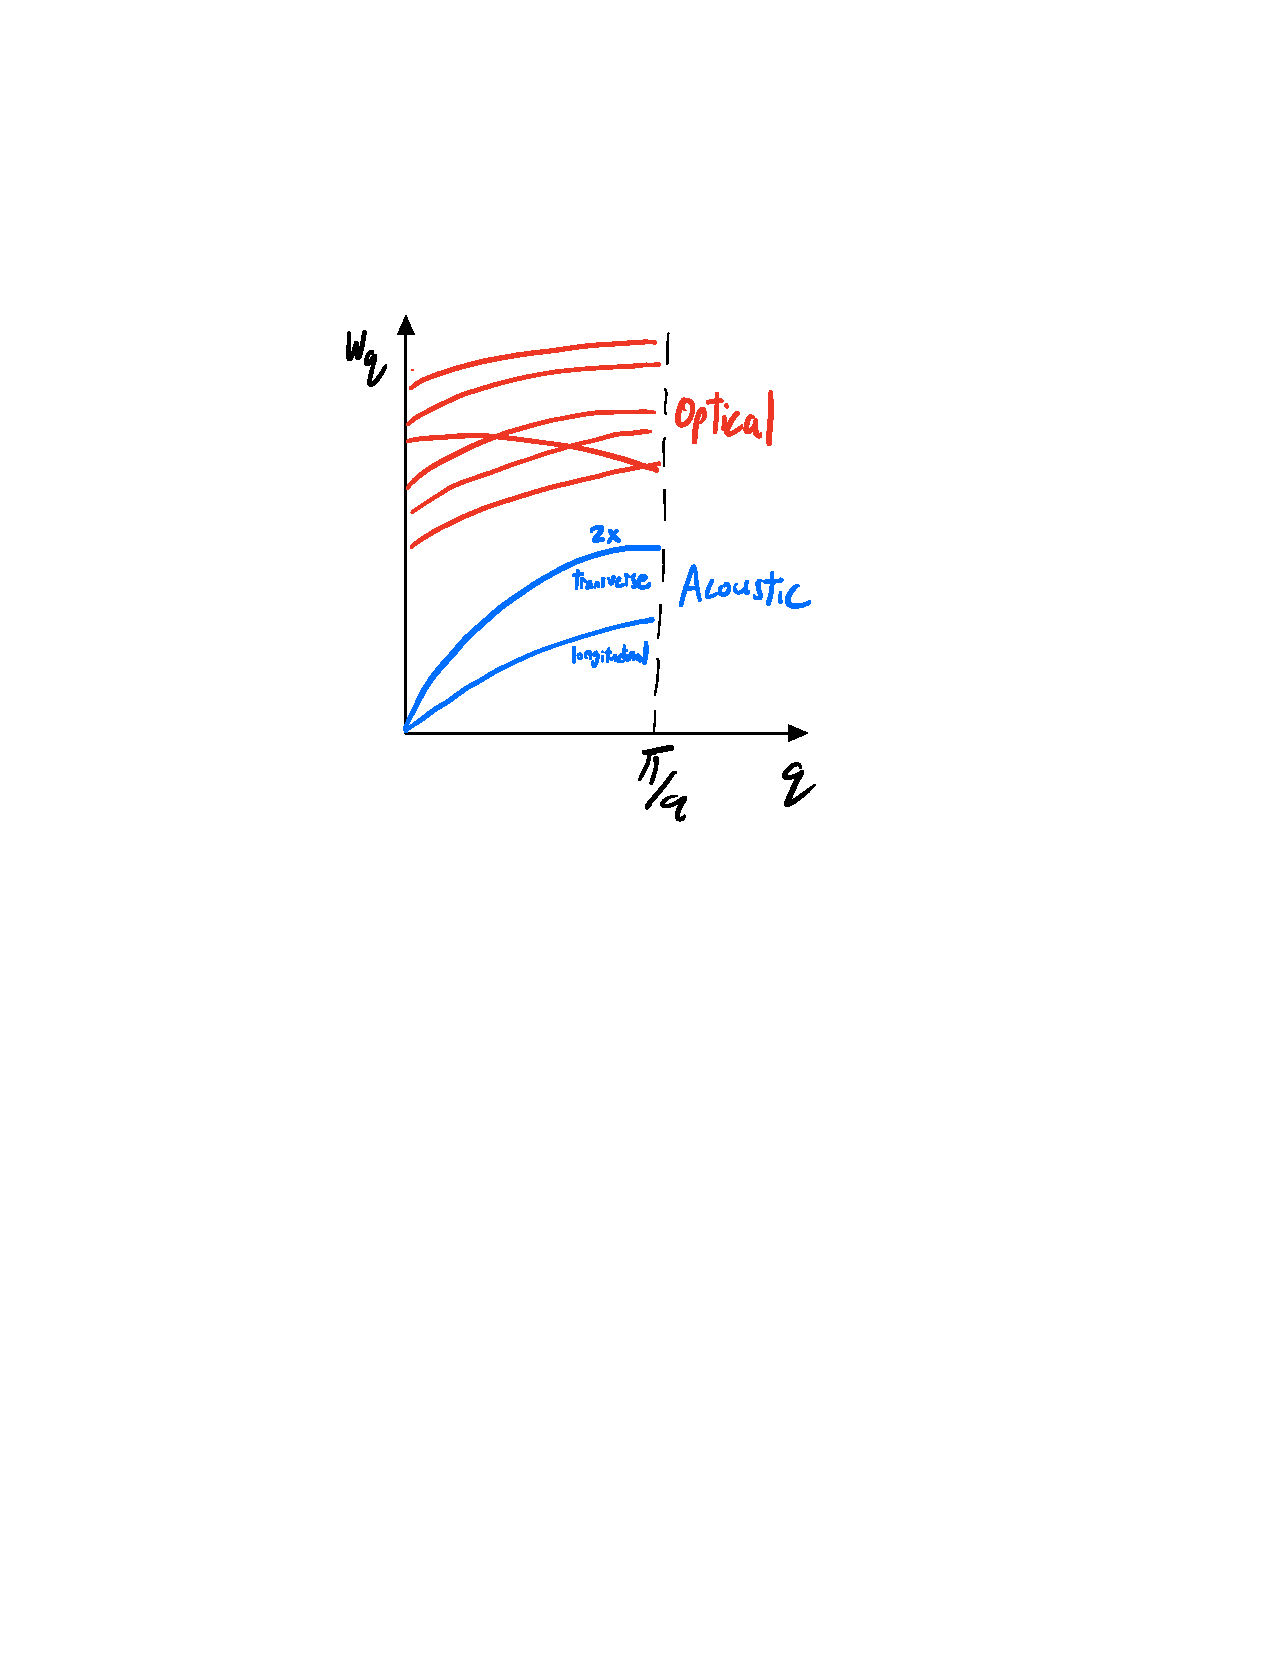
\includegraphics[scale=0.7]{Images/fig-3dphonondispersion.pdf}

    \caption{Plot of the phonon dispersion curves for a complex 3d solid. We have 3 acoustic modes (1 longitudinal mode and 2 degenerate transverse modes) and $3(n_d - 1)$ optical modes. }
    \label{fig-3dphonondispersion}
\end{figure}

\subsection{Debye Model, Specific Heat of Phonons}
This was one of the main puzzles in solid-state physics before the advent of QM! Let's figure out how to calculate this. The internal energy in lattice vibrations is given by:
\begin{equation}
    U = \avg{H}_\beta = \sum_{\v{q}\mu}\hbar \omega_{\v{q}\mu}(\avg{a^\dag_{\v{q}\mu}a_{\v{q}\mu}} + \frac{1}{2})
\end{equation}
Where $\avg{a^\dag_{\v{q}\mu}a_{\v{q}\mu}} = \bar{n}_{\v{q}\mu} = \frac{1}{e^{\beta \hbar \omega_{\v{q}\mu}} - 1}$ is the bose-einstein occupation factor. It will actually be easier to go straight to the heat capacity:
\begin{equation}\label{eq-photonCV}
    C_V = \dod{U}{T} = \frac{1}{k_B T^2}\sum_{\v{q}, \mu}\frac{(\hbar \omega_{\v{q}\mu})^2 e^{\beta \hbar \omega_{\v{q}\mu}}}{(e^{\beta\hbar\omega_{\v{q}\mu}} - 1)^2}
\end{equation}
to evaluate the sum we would need to know the form of $\omega_{\v{q}\mu}$, and even then there usually does not exist a closed-form solution for the summation.

To evaluate Eq. \eqref{eq-photonCV}, it is useful to define the phonon density of states:
\begin{equation}
    D(\omega) = \sum_{\v{q}, \mu} \delta(\omega - \omega_{\v{q}\mu})
\end{equation}
This implies:
\begin{equation}
    C_V = \frac{1}{k_BT}\int_0^\infty d\omega D(\omega)\frac{(\hbar\omega)^2 e^{\beta\hbar\omega}}{(e^{\beta\hbar\omega} - 1)^2}
\end{equation}
The Debye model assumes $\omega_{\v{q}\mu} = c_\mu\abs{\v{q}}$, approximating the acoustic modes as straight lines. It should be accurate at low $T$ when only low frequency acoustic phonons are thermally excited. For simplicity, we further assume equal velocities $c_\mu = c$ for $\mu = 1,2,3$ (but this is not essential, and the calculation can still be done). We then get:
\begin{equation}
    \begin{split}
        D(\omega) &= \frac{3V}{(2\pi)^3}\int d^3q \delta(\omega - cq)
        \\ &= \frac{3V}{(2\pi)^3}4\pi \int q^2 dq \delta(\omega - cq) 
        \\ &= \frac{3V}{3\pi^2}\frac{\omega^2}{c^3}.
    \end{split}
\end{equation}
where the $3$ comes from the 3 directions summed over and we evaluate the integral by going into spherical coordinates. 

\subsection{Debye Frequency, Momentum, Temperature}
There is one more constraint for us to accomodate. The density of states has the property that if we integrate over it, we should get the total number of modes in the entire system (which in this case should be $3N$; $N$ particles moving in three dimensions). Therefore, the above expression cannot go on forever; and this is evident from the acoustic spectra where we see there are no states above some energy. So, we introduce a Debye frequency $\omega_D$:
\begin{equation}
    D(\omega) = \begin{cases}
        \frac{3V}{2\pi^2}\frac{\omega^2}{c^3} & \Omega < \omega_D
        \\ 0 & \omega > \omega_D
    \end{cases}
\end{equation}
where $\omega_D$ is determined by:
\begin{equation}
    \int_0^{\omega_D}D(\omega)d\omega = 3N \implies \omega_D^3 = 4\pi^2c^3\frac{N}{V}
\end{equation}'

\begin{figure}[htbp]
    \centering
    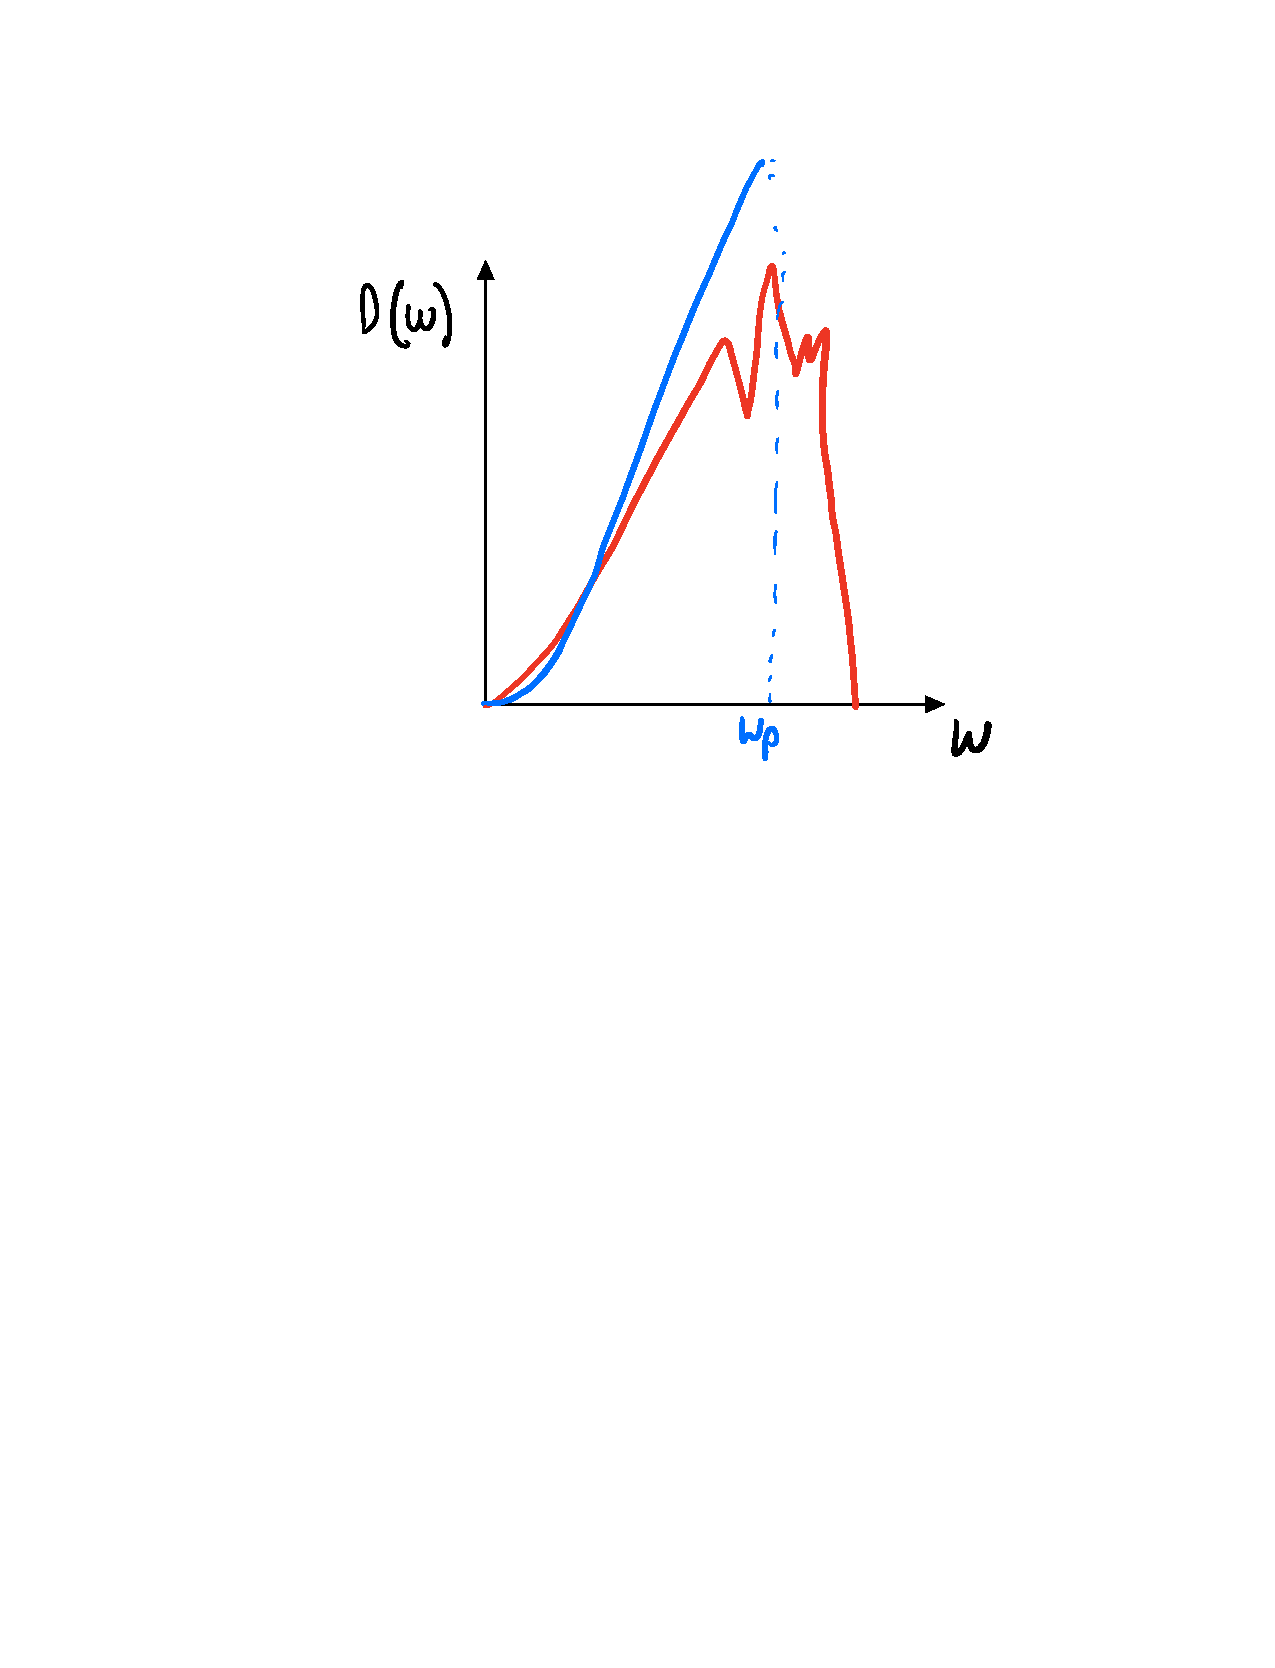
\includegraphics[scale=0.6]{Images/fig-phonondensityofstates.pdf}

    \caption{Plot of a realistic/experimentally measured phonon density of states (red) and our approximate calculated value (blue). We cut off the $\omega^2$ prediction for the density of the states at the Debye frequency $\omega_D$ such that the area under the curve (i.e. the total number of modes) is $3N$ (and the same for the two plots). It may seem like we neglect a lot of structure in making our approximation, but since we are itnerested in the heat capacity $C_V$, this complex structure generally gets smeared out regardless; hence our approximation can give reasonable predictions for heat capacity.}
    \label{fig-phonondensityofstates}
\end{figure}

This notion of a Debye frequency turns out to be very useful. It also defines Debye momentum:
\begin{equation}
    k_D = \frac{\omega_D}{c} = \left(6\pi^2\frac{N}{V}\right) \sim \frac{4}{a}
\end{equation}
where $a$ is the lattice spacing. It also defines the Debye temperature:
\begin{equation}
    \Theta_D = \frac{\hbar\omega_D}{k_B} \sim 74\si{K} - 1800\si{K}
\end{equation}
where $74\si{K}$ corresponds to Pr and $1800\si{K}$ corresponds to diamond. On average it is on the order of a few hundred Kelvin. These are all characteristic scales of phonons. Of all of them, Debye temperature tends to be the most useful as it is in the most tangible units. It distinguishes a low and high temperature regime for phonon excitations (i.e. the frequency for which below it the acoustic approximation is reasonable)

\subsection{Back to Heat Capacity}
We have:
\begin{equation}
    \begin{split}
        C_V &= \frac{3V\hbar^2}{2\pi^2c^2k_BT^2}\int_0^{\omega_B}d\omega \frac{\omega^4 e^{\beta\hbar\omega}}{(e^{\beta\bar\omega} - 1)^2}
        \\ &= gNk_B\left(\frac{T}{\theta_D}\right)^3\int_0^{\theta_D/T} dx \frac{x^4e^x}{(e^x - 1)^2}
    \end{split}
\end{equation}
where we have made the substitution $x = \beta\hbar\omega$. We call the integral $f(\theta_D/T) = f(x_D)$ the Debye function.

We now analyze some consequences. In principle we can solve the integral numerically, but we can also start by studying the integral analytically in two limits.

\subsubsection{Low T behavior}
In this limit we have $T \ll \theta_D$ and hence $x_D = \frac{\theta_D}{T} \gg 1$. We can therefore write:
\begin{align*}
    f(x_D) = \int_0^\infty \frac{x^4 e^x}{(e^x - 1)^2} - \int_{x_D}^\infty \frac{x^4 e^x}{(e^x - 1)^2} \approx \frac{4\pi^4}{15} - \int_{x_D}^\infty x^4 e^{-x} \approx \frac{4\pi^4}{15}
\end{align*}
where we have evaluated the first term analytically (calculus exercise) and the second integral we have that $x \gg 1$ over the rande of integration and we may therefore approximate $\frac{x^4e^x}{(e^x - 1)^2} \approx x^4 e^{-x}$. Since this is an exponentially small term, we can drop it. The specific heat then becomes:
\begin{equation}
    C_V \approx \frac{12\pi^4}{5}Nk_B\left(\frac{T}{\theta_D}\right)^3
\end{equation}
so for $T \ll \theta_D$ we find $C_V \sim T^3$. This is obeyed in many solids.

\subsubsection{High T behavior}
In this limit, we have $T \gg \theta_D$ and so $x_D \ll 1$. We therefore may expand $e^x$ to leading order in the integrand. This yields:
\begin{align*}
    f(x_D) \approx \int_0^{x_D}dx \frac{x^4}{(1+x-1)^2} = \int_0^{x_D} dx x^2 = \frac{1}{3}x_D^3
\end{align*}
where in the numerator we have approximated $e^x \sim 1$ and in the numerator we have approximated $e^x \sim 1 + x$.

So plugging this back into our specific heat expression:
\begin{equation}
    C_V \approx 3Nk_B
\end{equation}
so for $T \gg \theta_D$ we find that $C_V$ is independent of temperature. This is the Dulong-Petit law; this is the heat capacity of a harmonic crystal in classical theory (i.e. no quantum effects). If we recall the equipartition theorem, we have $N$ atoms oscillating in $3$ directions, so $3$ vibrational degrees of freedom and $3$ kinetic degrees of freedom and so $6N$ degrees of freedom in total. Equipartition associates $\frac{1}{2}k_B T$ per energy per degree of freedom and so we have $U = 6N \cdot \frac{1}{2}k_B T = 3Nk_B T$ of energy and hence $C_V = 3Nk_B$ specific heat. This of course in some sense makes sense as at high temperatures we expect quantum effects to be washed out and the system behaves basically classically (though an interesting point to note here - the quantum effect of the suppression of specific heat persists up to room temperature, as $\theta_D$ is on the order of hundreds of Kelvin; we do not have to cool our system to very low temperature for the quantum effects to become significant). This was known before QM was invented, but disagreed with experiment, where the specific heat went to zero at zero temperature (though it described the high-$T$ behavior well). With quantum mechanics, we are able to obtain a prediction that described experimental results very well.

\begin{figure}[htbp]
    \centering
    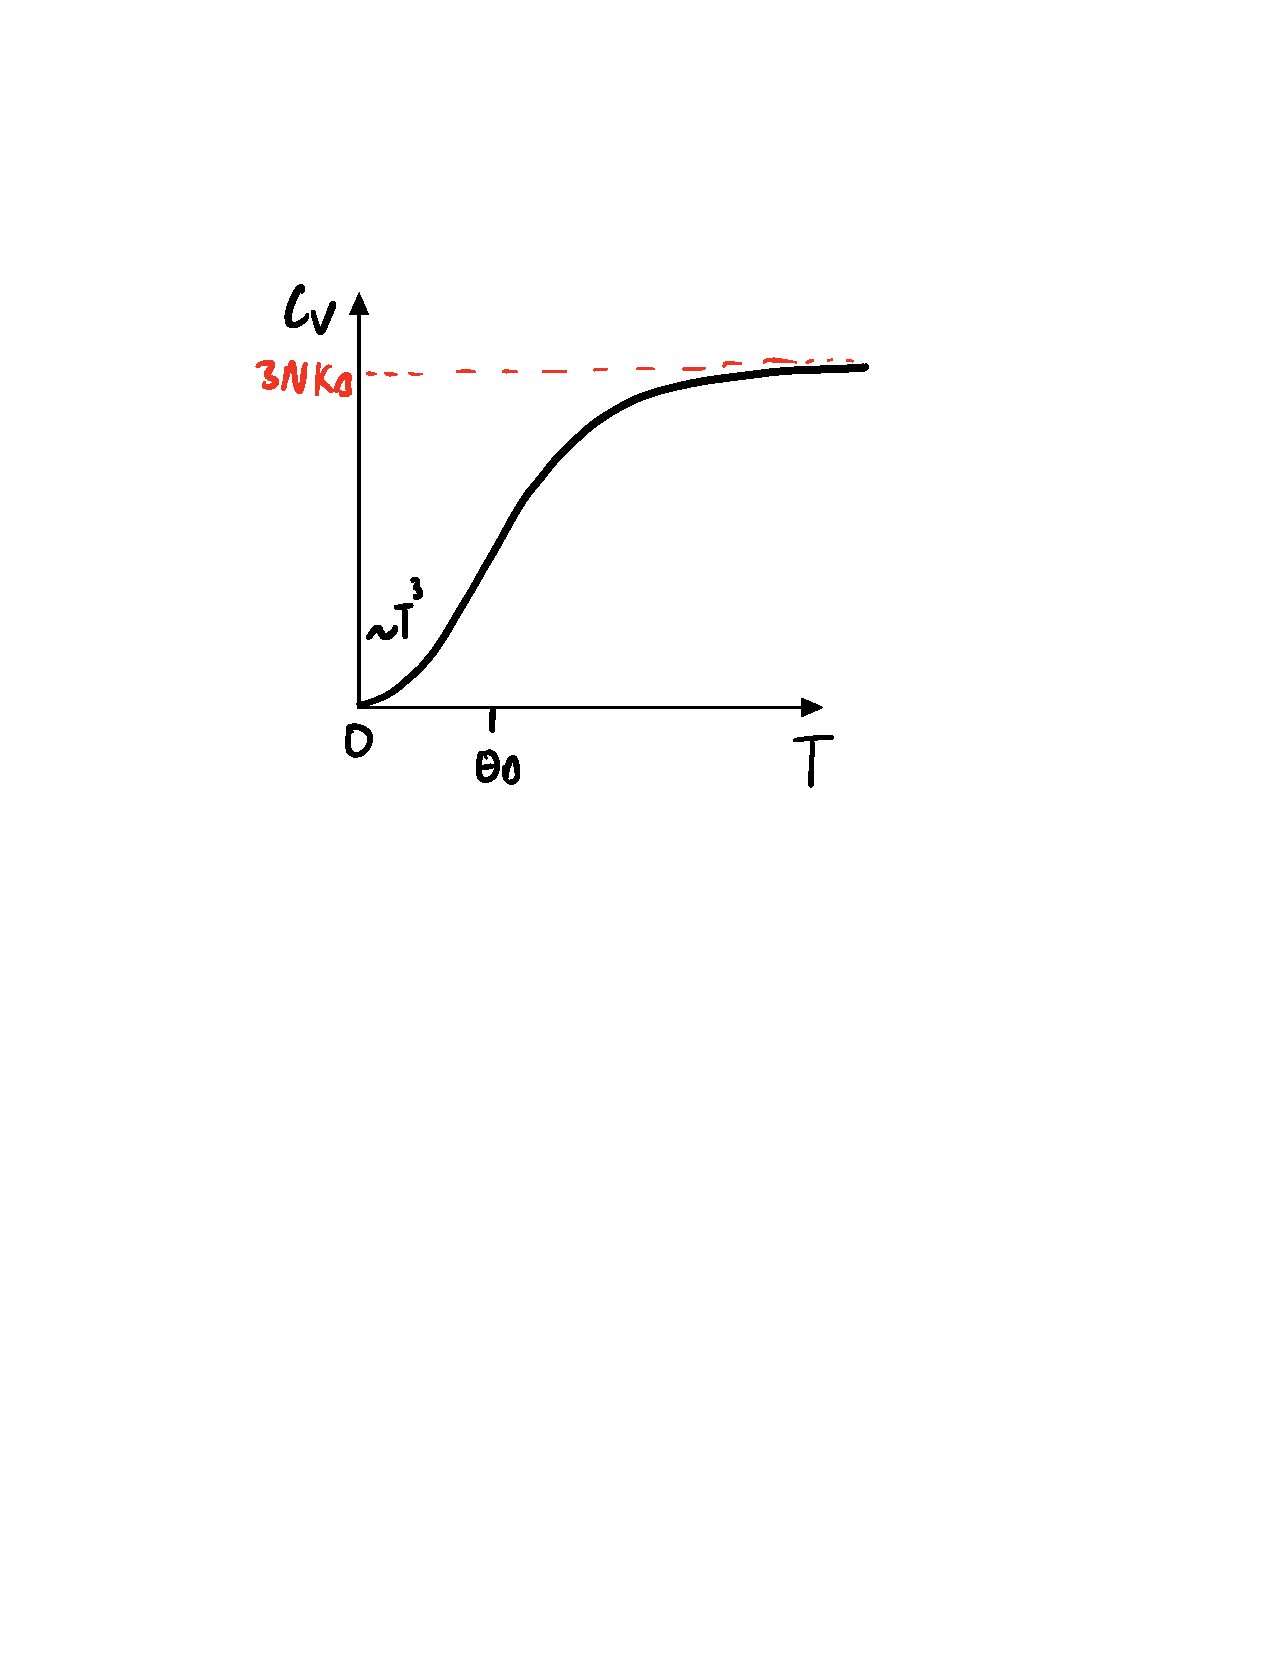
\includegraphics[scale=0.7]{Images/fig-phononspecificheat.pdf}

    \caption{Specific heat for phonons as a function of temperature $T$. At low $T$ we see $C_V \sim T^3$ behavior. At high $T$ we see that $C_V$ tends to a constant of $3Nk_B$.}
    \label{fig-phononspecificheat}
\end{figure}

\subsection{Einstein Model}
Is a model suitable for the study of optical phonons. We replace the dispersion relation for an optical phonon with an average $\omega_0$.

\begin{figure}[htbp]
    \centering
    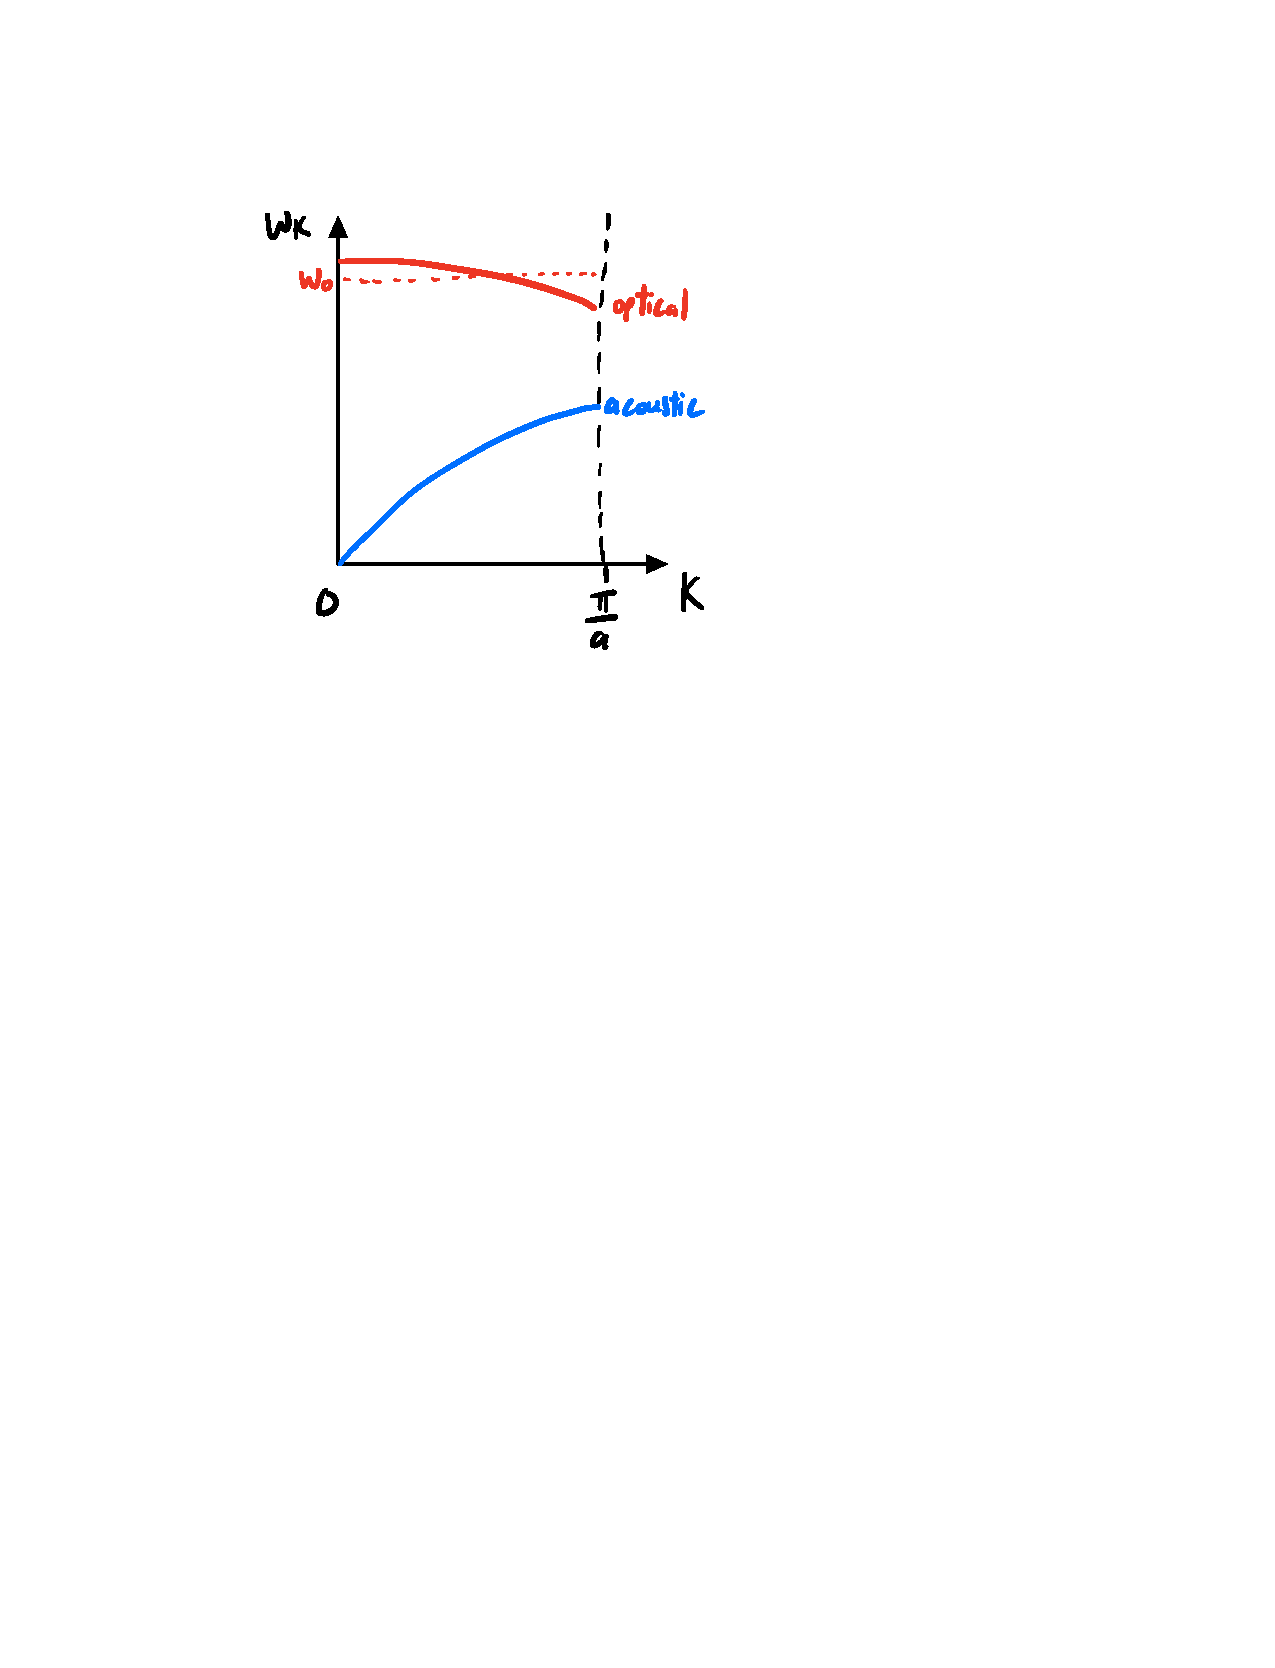
\includegraphics[scale=0.7]{Images/fig-einsteinmodelapprox.pdf}

    \caption{Dispersion relation for acoustic and optical modes of phonons, and Einstein's approximation for replacing the optical mode dispersion relation with a straight line at the average $\omega_0$.}
    \label{fig-einsteinmodelapprox}
\end{figure}


We consider an approximate phonon density of states:
\begin{align*}
    D(\omega) = N\delta(\omega - \omega_0)
\end{align*}
and from this we can calculate contribute to the heat capacity:
\begin{equation}
    C_V = \frac{1}{k_B T^2}\int_0^\infty d\omega\frac{(\hbar\omega)^2 e^{\beta\hbar\omega}}{(e^{\beta\hbar\omega} - 1)^2}D(\omega) = \frac{N}{k_BT^2}\frac{(\hbar\omega_0)^2 e^{\beta\hbar\omega_0}}{(e^{\beta\hbar\omega_0} - 1)^2}
\end{equation}
At low $T$, we have $\beta\hbar\omega_0 \gg 1$ and so:
\begin{equation}
    C_V \approx N k_B\left(\frac{\hbar\omega_0}{k_B T}\right)^2 e^{-\frac{\hbar\omega_0}{k_B T}}
\end{equation}
so we have ``exponentially activated behavior'' here.

\begin{figure}[htbp]
    \centering
    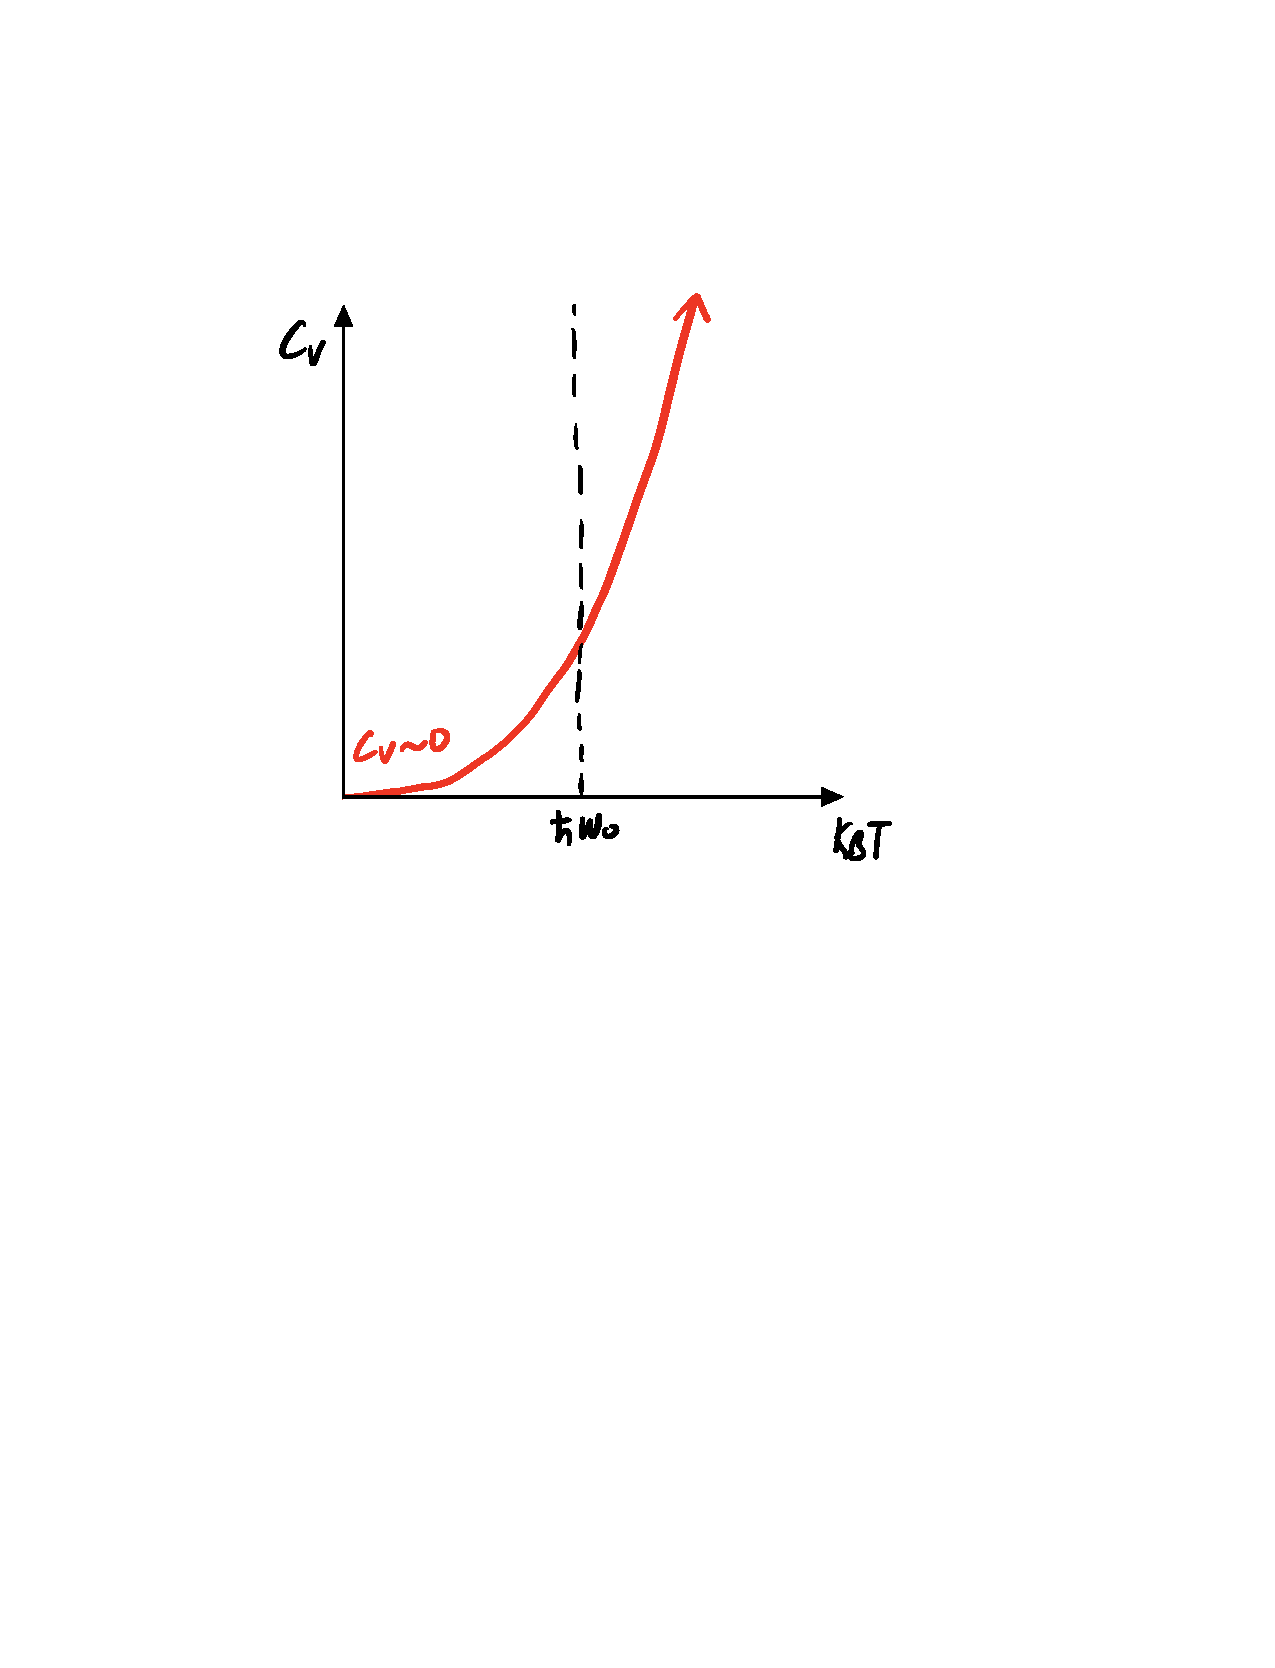
\includegraphics[scale=0.7]{Images/fig-einsteinmodelspecificheat.pdf}
    \caption{Plot of the low-$T$ specific heat as calculated by the Einstein model. We see the exponentially activated behavior, where past $\hbar\omega_0$ the specific heat sharply spikes.}
    \label{fig-einsteinmodelspecificheat}
\end{figure}

Interestingly, if we compare the two plots for the specific heat, they agree pretty well. Some differences at the very low $T$ limits, however. For the low $T$ einstein model at very low temperatures we do not even have one quantum of energy to excite, and so we have $C_V = 0$. Conversely, for the acoustic modes we are able to excite things at even very low temperatures (so long as the temperature is not zero).

\subsection{Anharmonic Effects and Phonon Interactions}
We take a step back and regard a solid (metal) as a collection of electrons (fermions) and phonons (bosons).

At low $T$, both the electrons and phonons contribute to thermodynamic (and other) properties, e.g. specific heat:
\begin{align*}
    C_V^{ph} \approx 6T^3 \text{ (Debye)}
\end{align*}
\begin{align*}
    C_V^{el} \approx aT \text{ (Sommerfield)}
\end{align*}
both are crucially quantum mechanical; if we forget quantum mechanics then these become temperature dependent constants. The total specific heat is the sum of the two:
\begin{align*}
    C_V = C^{el}_V + C^{ph}_V \approx aT + bT^3
\end{align*}
or:
\begin{equation}
    \frac{C_V}{T} \approx a + bT^2
\end{equation}
and many (most) metals behave in this way. This is a huge success of quantum theory and modern solid-state physics.

However, there are some significant failures of this model:
\begin{enumerate}
    \item Thermal expansion (Within the harmonic expansion, you can prove this does not occur)
    \item Thermal conductivity (Phonons to not carry heat in this model)
    \item Sound attenuation (Sound attenuates forever)
\end{enumerate}
but whenever our theories fail, we can look back to what approximations we have made, and see what things to improve. These three failures can be understood by incorporating anharmonic effects. In the harmonic approximation, we threw away all terms past the second derivative, but we could consider successive terms of order:
\begin{equation}
    H_3 = \frac{1}{3!}\sum_{RR'R''ijk}\mu_R^i \mu_{R'}^j \mu_{R''}^{k} V^{ijk}_{RR'R''}
\end{equation}
where:
\begin{equation}
    V^{ijk}_{RR'R''} = \left. \frac{\partial^3 V}{\partial \mu_R^i \partial \mu_{R'}^j \partial \mu_{R''}^k}\right|_{\mu=0}
\end{equation}

Note that the inclusion of these third-order terms is sufficient to describe thermal expansion and sound attenuation. To obtain thermal conductivity from the model, one needs to go to fourth order.

In translation-invariant systems, this can be expressed as:
\begin{equation}
    H_3 = \frac{1}{6\sqrt{N}}\left(\frac{\hbar}{2M}\right)^{3/2}\sum_{qq'q''ijk\mu\nu\lambda}\frac{S_\mu^i S_\nu^j S_\lambda^k}{(\omega_{q\mu}\omega_{q'\nu}\omega_{q''\lambda})^{1/2}}V^{ijk}_{qq'q''}\Delta (\v{q} + \v{q}' + \v{q}'') (a_{-q\mu}^\dag + a_{q\mu})(a^\dag_{-q'\nu} + a_{q'\nu})(a^\dag_{-q''\lambda} + a_{q''\lambda})
\end{equation}
This looks absolutely terrible, but people have come up with clever ways to analyze such Hamiltonians, namely through the graphical means of Feynman diagrams. Each of the product of three terms contains an annhilation and creation operator. If we were to multiply them out, we would get six terms, which could be represented as follows:


\begin{figure}[htbp]
    \centering
    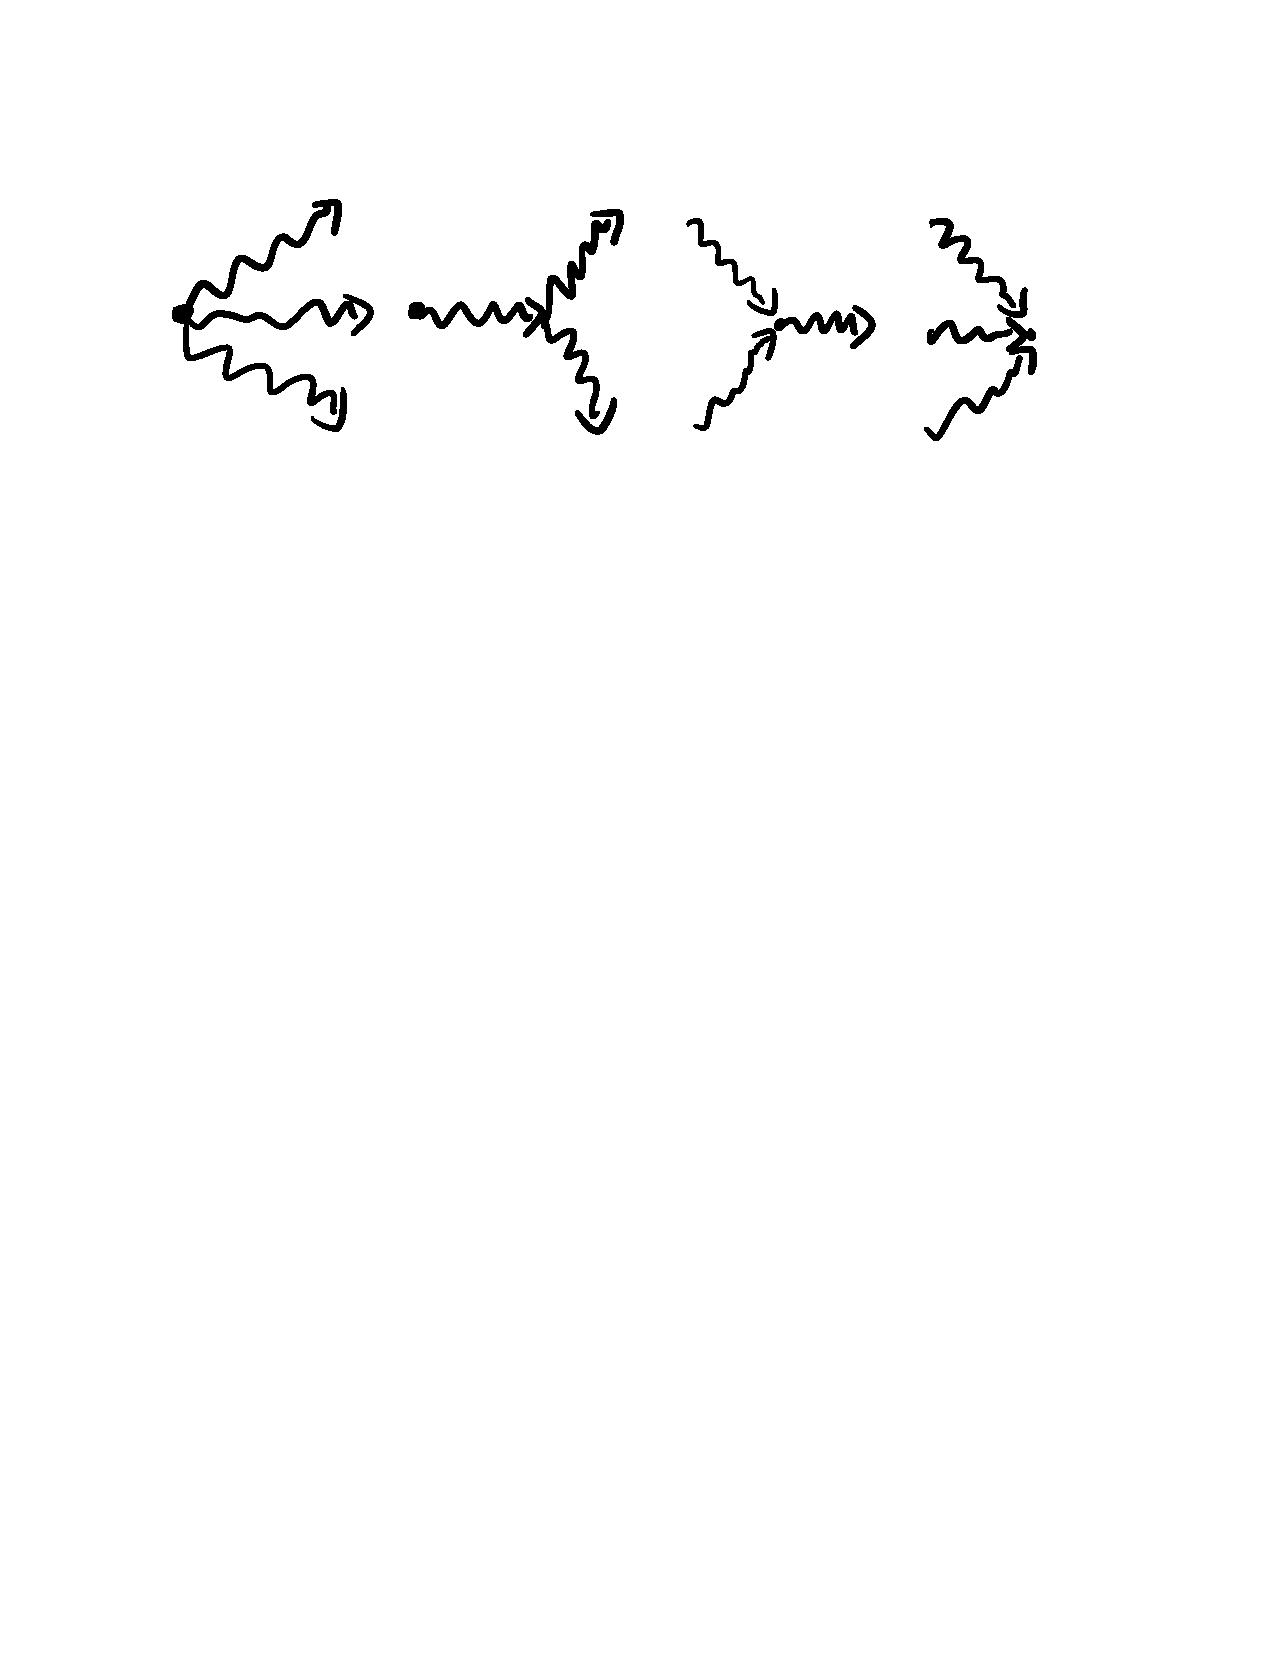
\includegraphics[scale=0.7]{Images/fig-threephonondiagrams.pdf}
    
    \caption{The four Feynman diagrams for three phonon interactions that come up in the third order term. In each diagram time runs from left to right. The leftmost diagram represents the creation of three phonons. The second diagram represents the destruction of one phonon and creation of two phonons. The third diagram represents the destruction of two phonons and creation of one phonon. Finally, the fourth diagram represents the destruction of three phonons.}
    \label{fig-threephonondiagrams}
\end{figure}

we can then assign a mathematical quantity to each of these diagrams, and thus evaluate each of their contributions in a clever way.

Without writing down the Hamiltonian, we can also look at the diagrams that arise in the fourth-order Hamiltonian $H_4$. We would have a product of four terms, which creates a sum with four phonons. Again, each of these diagrams could be assigned a mathematical quantity to evaluate their contribution.

\begin{figure}[htbp]
    \centering
    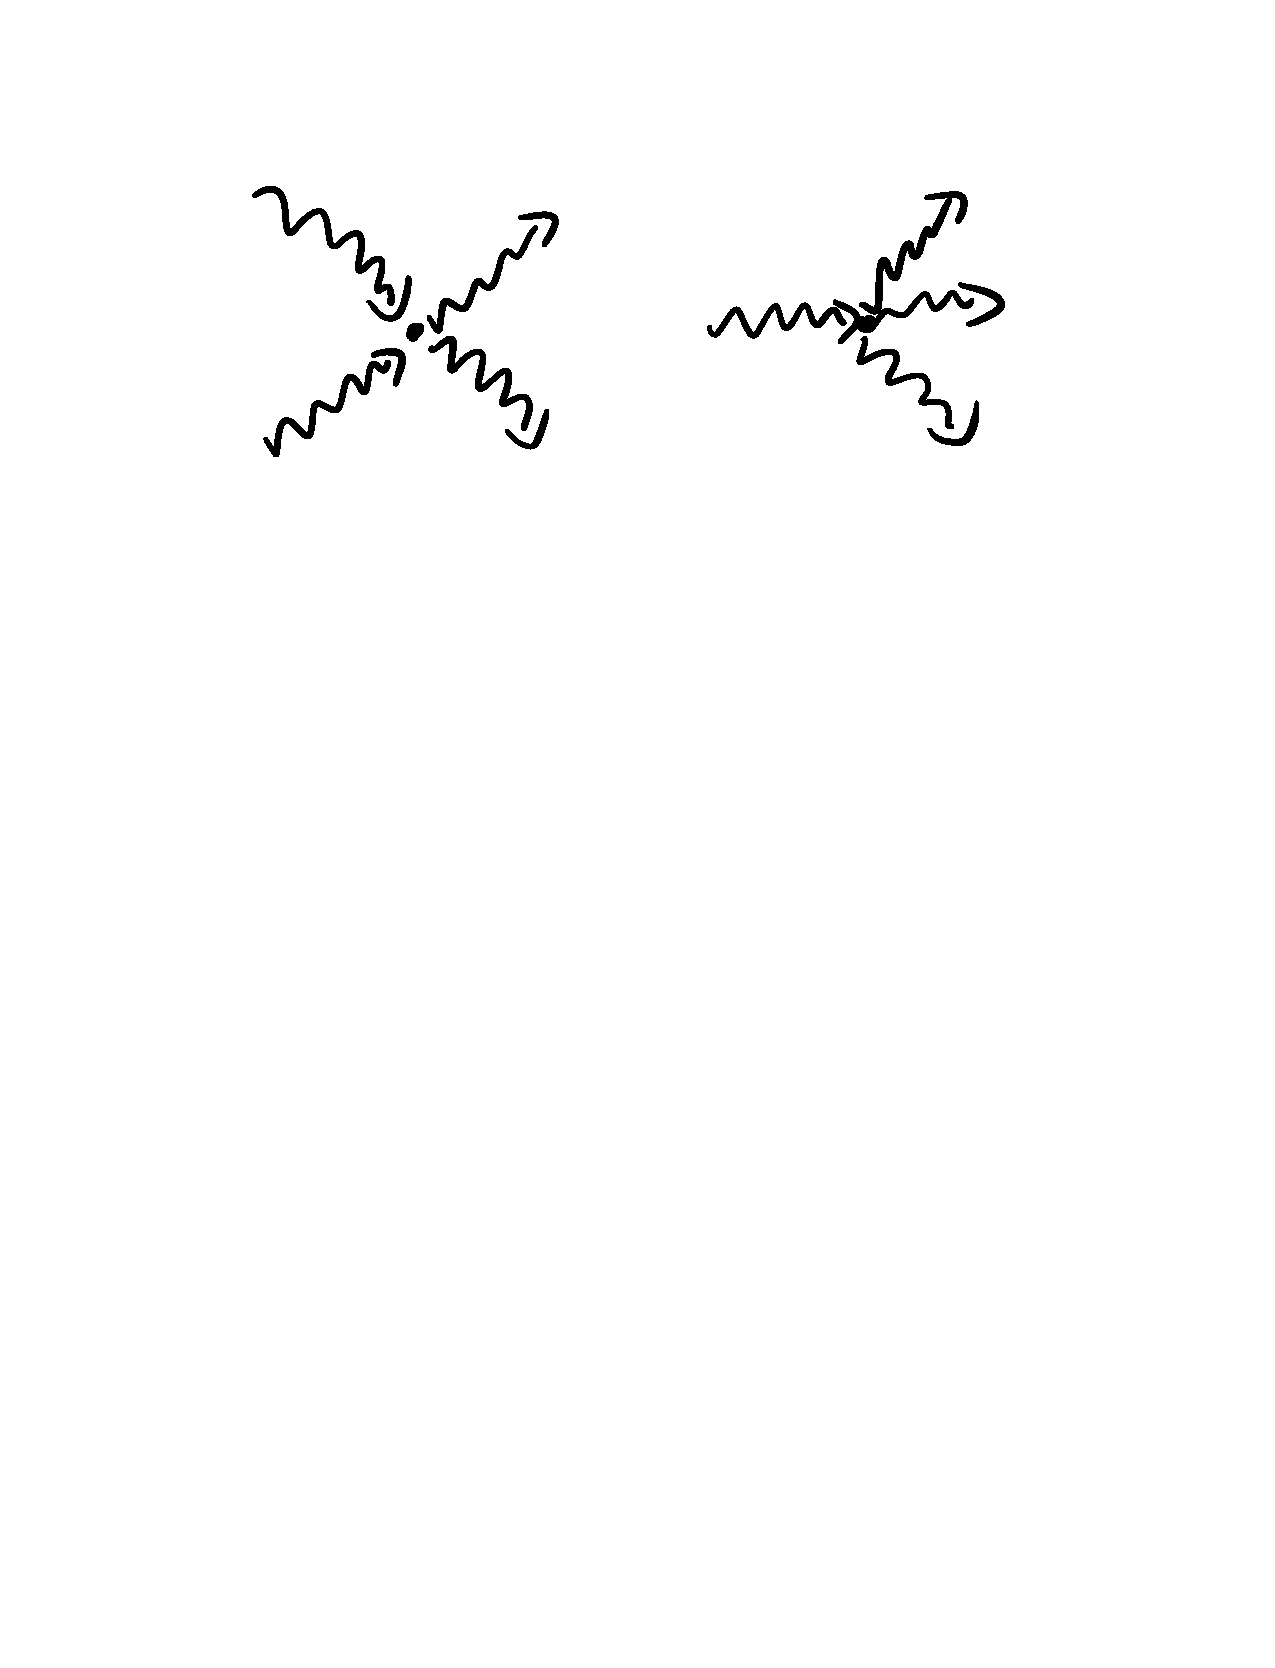
\includegraphics[scale=0.7]{Images/fig-fourphonondiagrams.pdf}
    
    \caption{Feynman diagrams for four phonon interactions that come up in the fourth order term. In each diagram time runs from left to right. The leftmost diagram represents the most dominantly contributing interaction, which is the scattering of two phonons. There are other interactions that also contribute, for example the destruction of one phonon and creation of three phonons as depicted in the right diagram.}
    \label{fig-fourphonondiagrams}
\end{figure}

\subsection{Thermal Conductivity}
In Drude theory, electrons contribute:
\begin{equation}
    \kappa_{el} = \frac{1}{3}C^{el}_V v_F l
\end{equation}
with $C^{el}_V$ the electronic specific heat, $v_F$ the Fermi velocity, and $l$ is the mean-free path - this is where many different details and factors come in (and generically very hard to calculate); this is where anharmonic effects enter. An electron that travelled forever would contribute an infinite conductivity - this does not happen so there must be features in our metal that slow it down, e.g. impurities. For phonons, we have (analogously)
\begin{equation}
    \kappa_{ph} = \frac{1}{3}C^{ph}_V c l'
\end{equation}
and again $l'$ the mean free path is where anharmonic effects enter (e.g. collisions of phonons with electrons).